\NeedsTeXFormat{LaTeX2e}
\documentclass[a4paper,12pt,
headsepline,           % Linie zw. Kopfzeile und Text
oneside,               % einseitig
pointlessnumbers,      % keine Punkte nach den letzten Ziffern in Überschriften
bibtotoc,              % LV im IV
%DIV=15,               % Satzspiegel auf 15er Raster, schmalere Ränder   
%BCOR15mm               % Bindekorrektur
%,draft
]{scrartcl}

\usepackage{amsmath}
\usepackage{amsfonts}
\usepackage{amssymb}
\usepackage{enumitem}
\usepackage[utf8]{inputenc} % this is needed for umlauts
\usepackage[ngerman]{babel} % this is needed for umlauts
\usepackage[T1]{fontenc} 
\usepackage{commath}
\usepackage{xcolor}
\usepackage{booktabs}
\usepackage{float}
\usepackage{tikz-timing}
\usepackage{tikz}
\usepackage{multirow}
\usepackage[final]{pdfpages}
\usepackage{blindtext}
\usepackage[scaled]{helvet}
\usepackage{hyperref}
\usepackage{comment}
\usepackage{mathtools}
\DeclarePairedDelimiter{\ceil}{\lceil}{\rceil}

\usetikzlibrary{calc,shapes.multipart,chains,arrows}

\KOMAoptions{DIV=last} % Neuberechnung Satzspiegel nach Laden von Paket helvet

\usepackage{scrpage2}
\pagestyle{useheadings}

\renewcommand{\familydefault}{\sfdefault} 

\setlength{\parindent}{0pt}   % kein linker Einzug der ersten Absatzzeile
\setlength{\parskip}{1.4ex plus 0.35ex minus 0.3ex} % Absatzabstand, leicht variabel

\newcommand{\fullname}{Gruppe 10}
\newcommand{\titel}{Softwaregrundprojekt Meilenstein 3}
\newcommand{\jahr}{2019}
\newcommand{\dozent}{Florian Ege}
\newcommand{\betreuer}{Stefanos Mytilineos}
\newcommand{\fakultaet}{Ingenieurwissenschaften, Informatik und\\Psychologie}
\newcommand{\institut}{Institut für Softwaretechnik und Programmiersprachen}

\pdfinfo{
    /Author (\fullname)
    /Title (\titel)
    /Producer     (pdfeTex 3.14159-1.30.6-2.2)
    /Keywords ()
}

\hypersetup{
    pdftitle=\titel,
    pdfauthor=\fullname,
    pdfsubject={Softwaregrundprojekt-Abgabe},
    pdfproducer={pdfeTex 3.14159-1.30.6-2.2},
    colorlinks=false,
    pdfborder=0 0 0	% keine Box um die Links!
}

% Trennungsregeln
\hyphenation{Sil-ben-trenn-ung}


\begin{document}
    \thispagestyle{empty}
    \begin{addmargin*}[4mm]{-10mm}

        
\includegraphics[height=1.8cm]{images/unilogo_bild}
        \hfill
        
\includegraphics[height=1.8cm]{images/unilogo_wort}\\[1em]

        {\footnotesize
        %{\bfseries Universität Ulm} \textbar ~89069 Ulm \textbar ~Germany
        \hspace*{115mm}\parbox[t]{35mm}{\bfseries Fakultät für\\
        \fakultaet\\
        \mdseries \institut}\\[2cm]

        \parbox{140mm}{\bfseries \LARGE \titel}\\[2.5em]
        {\footnotesize Softwaregrundprojekt an der Universität Ulm}\\[3em]

        {\footnotesize \bfseries Vorgelegt von:}\\
        {\footnotesize \fullname\\}\\ [1em]
        {\footnotesize \bfseries Dozent:}\\
        {\footnotesize \dozent\\}\\[1em]
        {\footnotesize \bfseries Betreuer:}\\
        {\footnotesize \betreuer}\\ [1em]
        {\footnotesize \jahr}
        }
    \end{addmargin*}
    \pagebreak
    \tableofcontents
    \pagebreak
    
    \section{Schnittstellenarten, Dialoge und Dialogstruktur}
    
    \subsection{Team- und Partiekonfigurator}
    
    Diese Komponente enthält einen Konfigurator, mit dem sich sowohl Quidditch-Teams, als auch Partien konfigurieren lassen.
	
	\subsubsection{Schnittstellenarten}
	
	Als Benutzerschnittstelle wird, wie im Lastenheft vorgeschrieben, eine GUI verwendet. \textbf{Begründung:} Der Nutzer möchte alle Informationen zu einer gegebenen Konfiguration übersichtlich dargestellt bekommen und anhand dieser Darstellung direkt Änderungen vornehmen können. Hierfür ist eine GUI die intuitivste und sinnvollste Variante, da eine grafische Darstellung eine übersichtliche Visualisierung erlaubt und eine Änderung direkt anhand dieser Visualisierung möglich ist. Zudem kann auf diese Weise die Komponente reibungslos in die Client-Anwendung integriert werden, was ebenfalls im Interesse des Nutzers ist.
	
	\subsubsection{Dialoge}
	
	Im Folgenden werden den bereits formulierten Anforderungen und Anwendungsfällen der Komponente den entsprechenden Dialogen zugeordnet.
	
	\begin{tabular}{| l l l l |}
	\hline
	\textbf{Name} & \textbf{Typ} & \multicolumn{2}{l|}{\textbf{Abgedeckte Anwendungsfälle}} \\\hline
	Konfiguratormenü & Dialog & QA18 & implizit aus Benutzerfreundlichkeit\\\hline
	Teammenü & Dialog & QA18 & implizit aus Benutzerfreundlichkeit\\\hline
	Team laden & Dialog & FA72 & Konfiguration öffnen \\\hline
	Teamkonfigurator & Dialog & FA70-72 & Konfiguration erstellen/bearbeiten\\\hline
	Team speichern & Dialog & FA72 & Konfiguration speichern \\\hline
	Partiemenü & Dialog & – & implizit, da Strukturierung erforderlich\\\hline
	Partiekonfiguration laden & Dialog & FA72 & Konfiguration öffnen \\\hline
	Partiekonfigurator & Dialog & FA70-72 & Konfiguration erstellen/bearbeiten\\\hline
	Partiefonfiguration speichern & Dialog & FA72 & Konfiguration speichern \\\hline
	Konfiguration erfolgreich & Popup & QA17-18 & Benutzerfreundlichkeit und Robustheit\\\hline
	Konfiguration ungültig & Popup & QA17-18 & Benutzerfreundlichkeit und Robustheit\\\hline
		
	\end{tabular}
	
	\subsubsection{Dialogstrukturdiagramme}    
	
	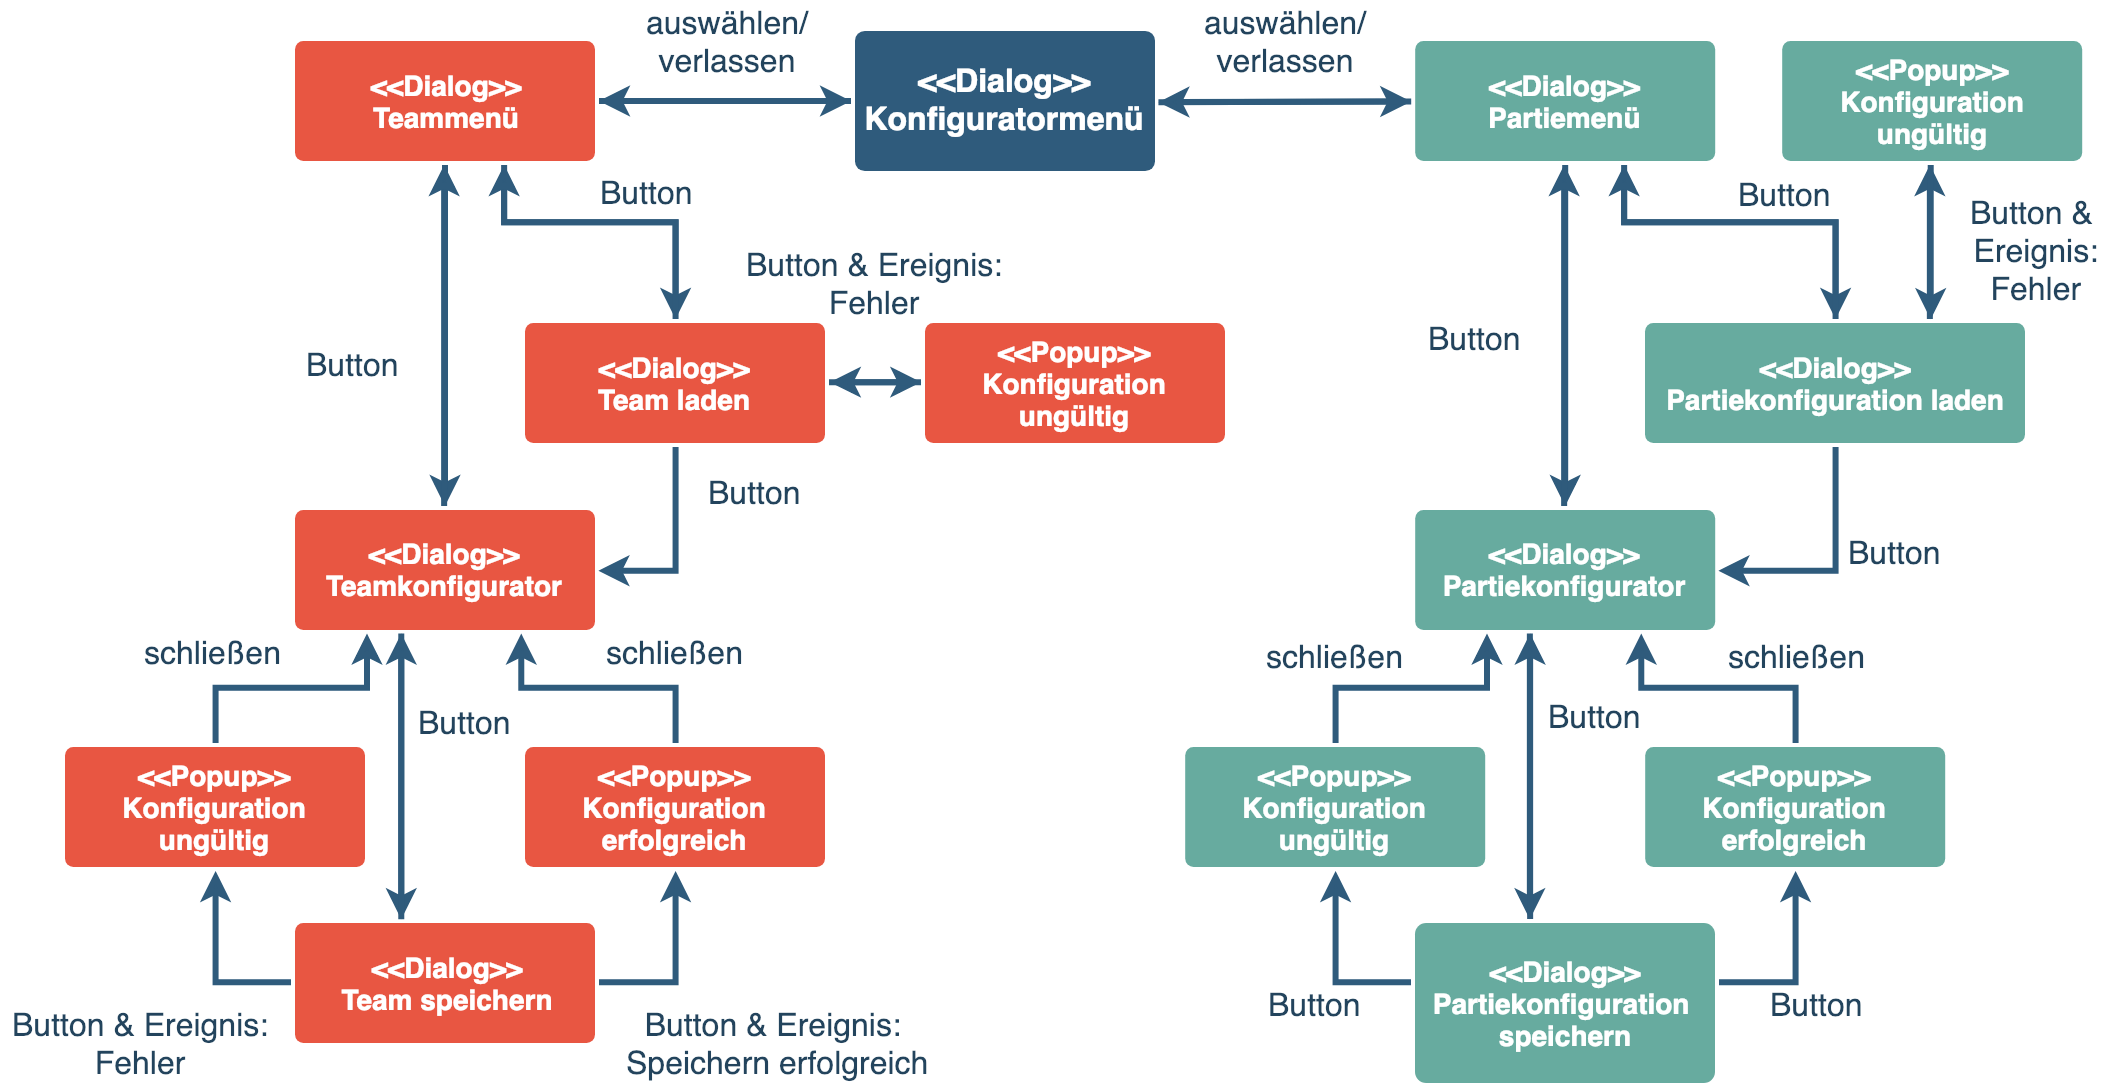
\includegraphics[width=15.5cm]{images/dialogstruktur_konfigurator}
	
	\section{Grafische Gestaltung und Nutzungskonzept}
	
	\subsection{Team- und Partiekonfigurator}
	
	\subsubsection{Konfiguratormenü}
	
	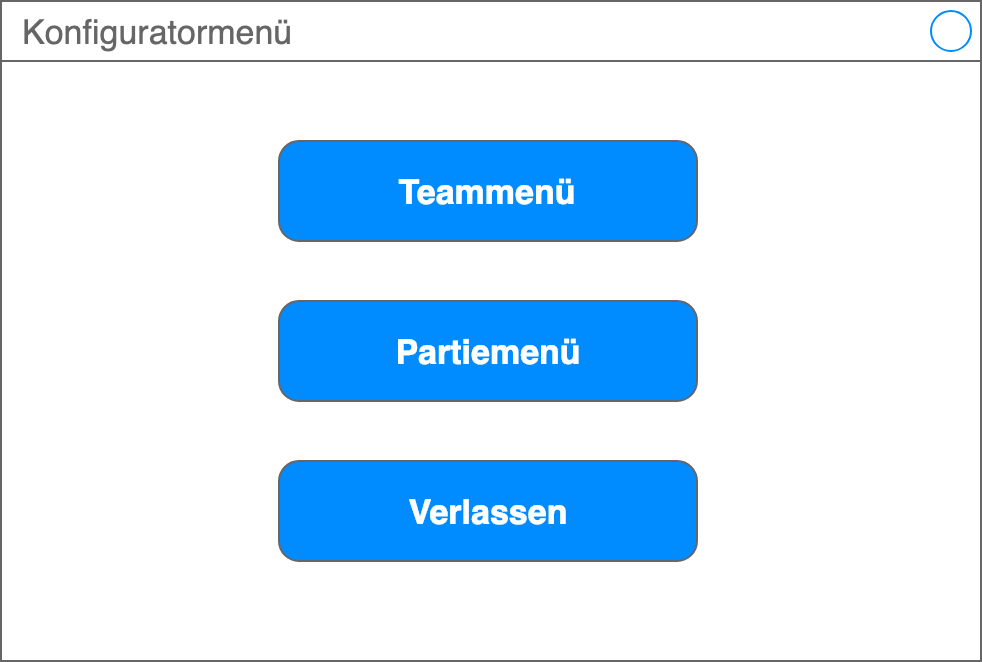
\includegraphics[scale=0.2]{images/konfiguratormenue}
	
	Über das Konfiguratormenü kann eine Auswahl zwischen dem Teammnü und dem Partiemenü über die entsprechenden Buttons getroffen werden. Diese führen zu den Menüs der jeweiligen Konfiguratoren. Über den Button \textit{Verlassen} kann der Konfigurator verlassen werden.
	
	\subsubsection{Teammenü}
	
	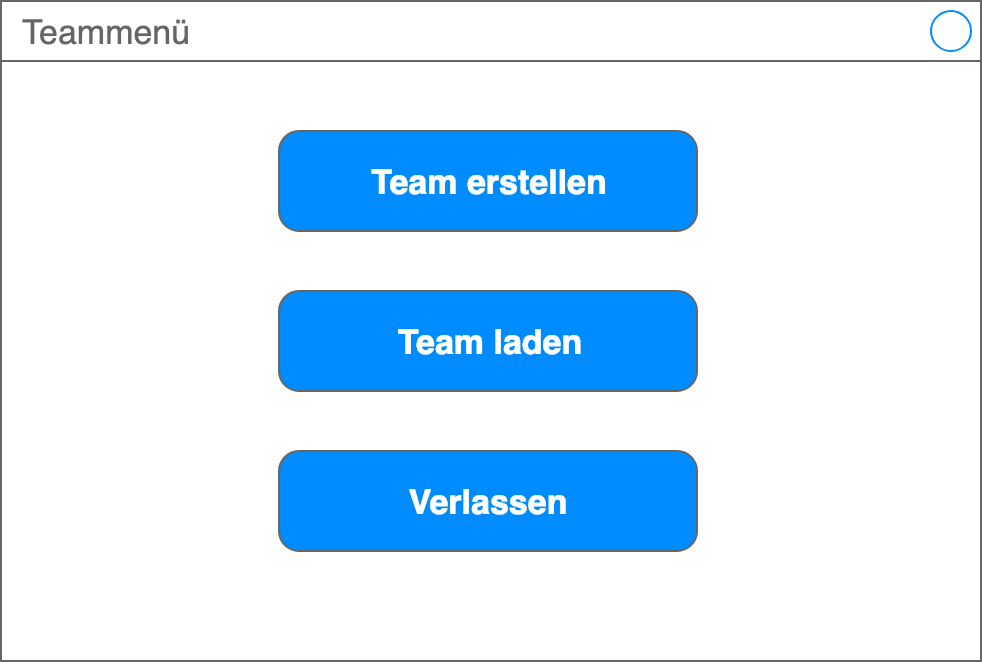
\includegraphics[scale=0.2]{images/teammenue}
	
	Über das Teammenü kann eine Auswahl zwischen dem Laden und dem Erstellen einer Teamkonfiguration getroffen werden. Das erfolgt über die entsprechenden Buttons. Über den Button \textit{Verlassen} kann das Teammenü verlassen werden.
	
	\subsubsection{Team bzw. Partiekonfiguration laden}
	
	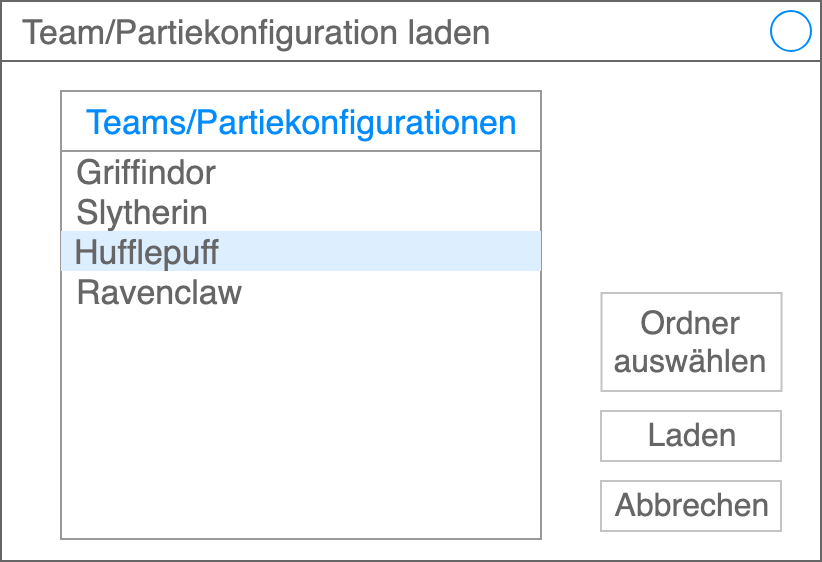
\includegraphics[scale=0.3]{images/laden}
	
	Über diesen Dialog kann eine bereits vorhanden Konfigurationsdatei ausgewählt und im Konfigurator geladen werden. Das erfolgt über ein Dateiauswahlelement und die entsprechenden Buttons. Über den Button \textit{Abbrechen} gelangt man zurück zu den entsprechenden Menüs. Da das Laden einer Teamkonfiguration nahezu identisch zum Laden einer Partiekonfiguration ist, wurde diese beiden Fälle in einem zusammen gefasst. Sollte eine zu ladende Konfigurationsdatei ungültig sein, öffnet sich das Popup \textit{Konfiguration ungültig}.


	\subsubsection{Teamkonfigurator}
	
	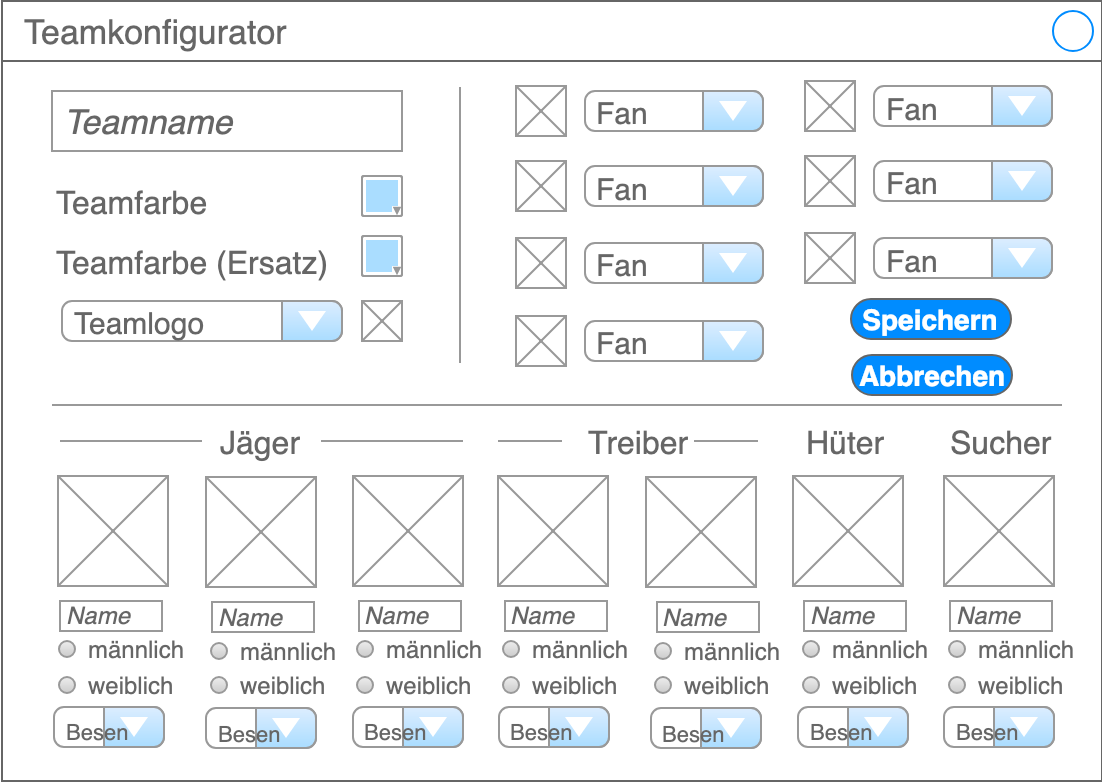
\includegraphics[scale=0.4]{images/teamkonfigurator}
	
	Im Teamkonfigurator können alle Paramter eines Teams eingestellt werden. Team- und Spielernamen lassen sich durch ein Textfeld bearbeiten. Teamfarben sind über eine Farbauswahl einstellbar. Das Teamlogo lässt sich aus einer Liste vorhandener Logos auswählen. Fans sowie Besen der Spieler sind über eine Dropdown-Auswahl einstellbar. Das Geschlecht der Spieler lässt sich über Radio-Buttons einstellen. Bei jeder Änderung werden die entsprechenden Bedingungen für eine gültige Konfiguration geprüft und der Nutzer erhält visuelles Feedback (z. B. in Form von roter Schriftfarbe in den entsprechenden Feldern). Über den Button \textit{Abbrechen} lässt sich der Konfigurator jederzeit verlassen. Ist eine gültige Auswahl eingestellt, kann die Konfiguration über \textit{Speichern} in einem separaten Speicherdialog persistiert werden.
	
	\subsubsection{Team bzw. Partiekonfiguration speichern}
	
	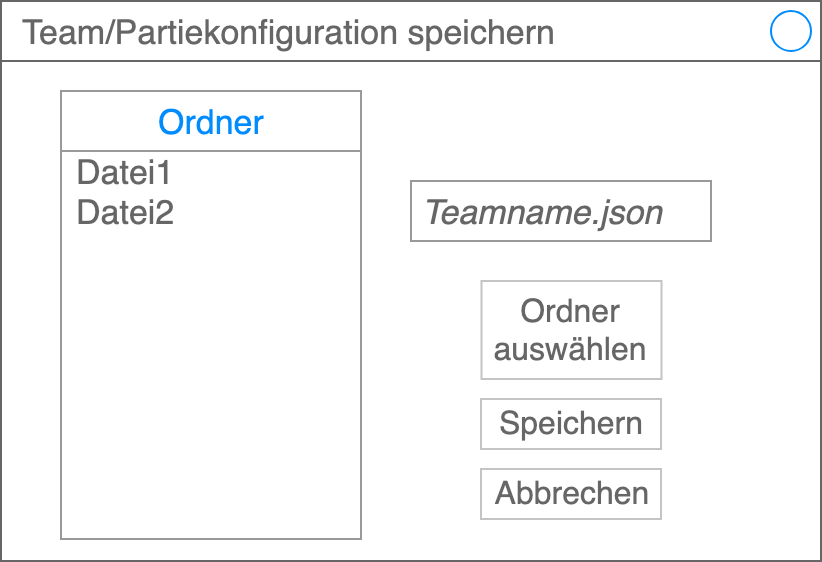
\includegraphics[scale=0.3]{images/speichern}
	
	In diesem Dialog kann Dateiname und Speicherort der Konfiguration festgelegt werden. Der Button \textit{Abbrechen} bringt den Nutzer direkt zurück in den entsprechen Konfigurator. Durch Klicken auf den Button \textit{Speichern} wird die Datei mit dem gewählten Namen und Speicherort gespeichert.
	
	Wurde versucht eine Konfiguration mit ungültigen Parametern zu speichern oder trat beim Speichervorgang irgend ein anderer Fehler auf, wird der Nutzer über dieses Popup darüber informiert. Der \textit{Ok}-Button führt zurück zum entsprechenden Konfigurator.
	
	\subsubsection{Konfiguration erfolgreich}
	
	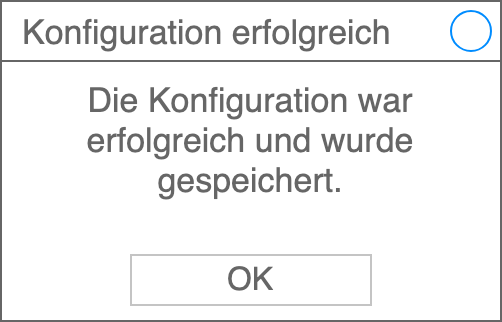
\includegraphics[scale=0.2]{images/konfiguration_erfolgreich}
	
	Wenn alle Paramter einer Konfiguration gültig waren, wird dieser Dialog angezeigt. Der \textit{Ok}-Button führt zurück zum entsprechenden Menü.
	
	\subsubsection{Konfiguration ungültig}
	
	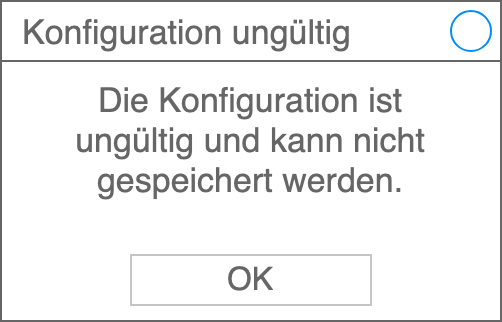
\includegraphics[scale=0.2]{images/konfiguration_ungueltig}
	
	Wurde versucht eine Konfiguration mit ungültigen Parametern zu speichern oder trat beim Speichervorgang irgendein anderer Fehler auf, wird der Nutzer über dieses Popup darüber informiert. Der \textit{Ok}-Button führt zurück zum entsprechenden Dialog.
	
	\subsubsection{Teammenü}
	
	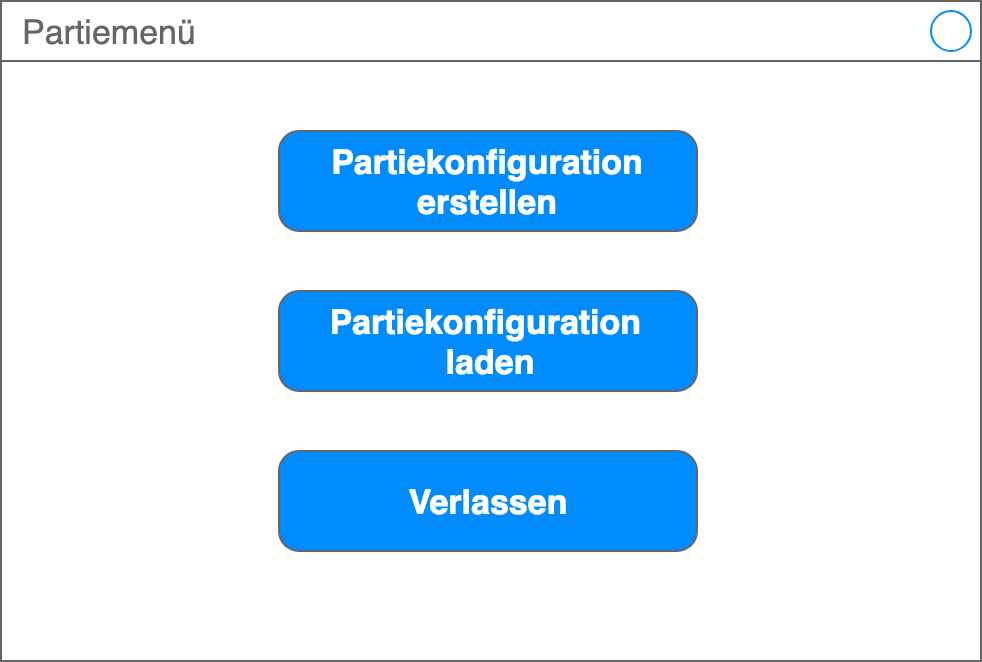
\includegraphics[scale=0.2]{images/partiemenue}
	
	Über das Partiemenü kann eine Auswahl zwischen dem Laden und dem Erstellen einer Partiekonfiguration getroffen werden. Das erfolgt über die entsprechenden Buttons. Über den Button \textit{Verlassen} kann das \texit{Partiemenü} verlassen werden.
	
	\subsubsection{Teamkonfigurator}
	
	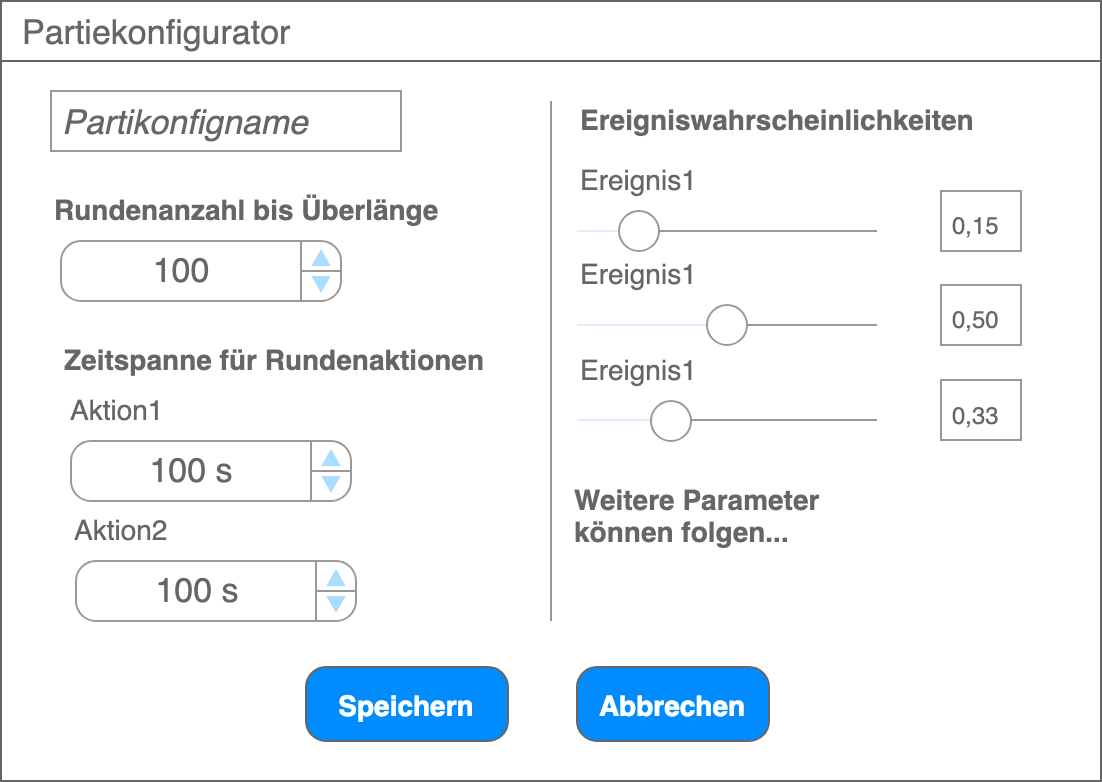
\includegraphics[scale=0.4]{images/partiekonfigurator}
	
	Im Partiekonfigurator können alle Paramter für eine gültige Teamkonfigurationsdatei eingestellt werden. Dazu gehören unter anderem die Rundenzahl, bis Überlänge erreicht ist, die Zeitspannen für die jeweiligen Spielaktionen und Ereigniswahrscheinlichkeiten. Je nach Art des Parameteres sind Spinner, Slider, Textfelder oder im weiteren Verlauf der Implementierung noch andere Auswahlelemente vorhanden.
	
	Über den Button \textit{Speichern} gelangt man in den \textit{Partiekonfiguration speichern}-Dialog. Der Button \textit{Abbrechen} führt zurück ins \textit{Teammenü}.
	
   
\end{document}
